
\chapter{The ``software crisis'' and encapsulation}

This book is going to dive deeply into a huge pile of nuts and bolts. But
before we take the leap into particulars, it's important to stand briefly at
the precipice and understand why we're jumping. What does ``object-oriented''
mean? What problem was it intended to solve? When was it invented and why?

\section{Ancient history}

A long time ago, in our own galaxy, a situation emerged which has been labeled
\textbf{the software crisis}. This crisis didn't happen at an instant in time;
it was a set of disagreeable circumstances which gradually evolved until it
became unbearable. The crisis is usually dated somewhere in the 1970's. This
was just as the high-tech computing industry was really starting to heat up,
on its way to permanently changing the lives of almost everyone on the planet.

Now ``crisis'' is an alarming word, designed to get your attention. It's worth
asking what all the hubbub was about. The immediate symptom may not strike you
as a three-alarm fire: it was simply that software projects were tending to
overrun their schedules.

The '70's were not a very plug-and-play era, since standards had not yet
evolved to facilitate intercompatibilities between devices or programs. So the
focus was often on building complete systems from the ground up. Engineering
teams would plan releases of key product lines that involved numerous
components, such as system architecture, hardware design and integration, data
collection and organization, system and network configuration, and software
development at both the operating system and the end user levels.

What managers discovered was that consistently, the \textit{software}
components of projects were coming in late and over-budget. Sometimes, they
didn't get finished at all. When they did, they were buggy and brittle. And
they were especially vulnerable to requirements changes: if circumstances were
discovered during the project that required a change in the way the software
needed to work, the software team was often strikingly unable to adapt to
this. They could be set back weeks or months to implement even a modest
change.

This astonished everyone at the time. After all, ``\textit{soft}ware'' -- a
pun on ``hardware'' -- was a term intended to convey the flexible, malleable
nature of computer programs as contrasted with physical devices. Software was
supposed to be easy to write and easy to change. That was the point. You
didn't need complex manufacturing processes: you needed a desktop computer and
a text editor. And you (seemingly) didn't face challenges of scale the way you
did with hardware: you could run out of room to put logic circuits on a chip
or a motherboard, but there was no limit to the size of a text file. 

So building complex stuff quickly, and turning on a dime when necessary, ought
to be easy to do in software. Right?

\subsection{Quantifying the crisis}

\begin{figure}[ht]
\centering
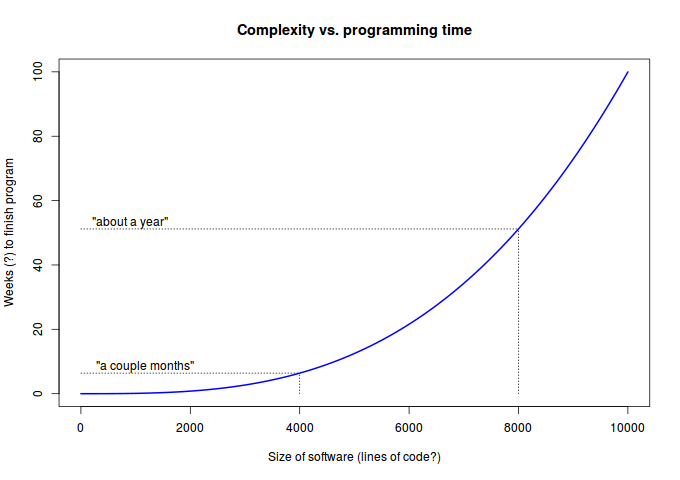
\includegraphics[width=0.7\textwidth]{complexityCurve.png}
\caption{The software crisis quantified: how long it took to complete a
program of various sizes. (Conceptual.)}
\label{fig:complexityCurve}
\end{figure}

\section{Software and complexity}

% The software crisis

% "soft"ware
% time vs. complexity curve

% Programming language diagram

\section{Dependencies}

\section{Encapsulation}

\section{Features of OO}

\section{Exercises}

Use an index card or a piece of paper folded lengthwise, and cover up the
right-hand column of the exercises below. Read each exercise in the
left-hand column, answer it in your mind, then slide the index card down to
reveal the answer and see if you're right! For every exercise you missed,
figure out why you missed it before moving on.

\begin{small}
\begin{enumerate}
\newcolumntype{Q}{>{\arraybackslash}m{.3\textwidth}}
\newcolumntype{A}{>{\arraybackslash}m{.6\textwidth}}
%\begin{longtable}{m{0.3\textwidth} || m{0.6\textwidth}}
\begin{longtable}{Q || A}
\hline
\item 
What key software problem was the OO paradigm invented to address?
&
Too many dependencies.
\\
\hline

\end{longtable}
\end{enumerate}
\end{small}
